\hypertarget{P45}{}
\begin{solution}{normal} % 45
In the circuit shown below, all capacitors are initially uncharged. a) Find the current through the battery immediately after closing switch $K$. b) What will be the charges on each of the capacitors after a steady state has been reached?
\begin{center}
    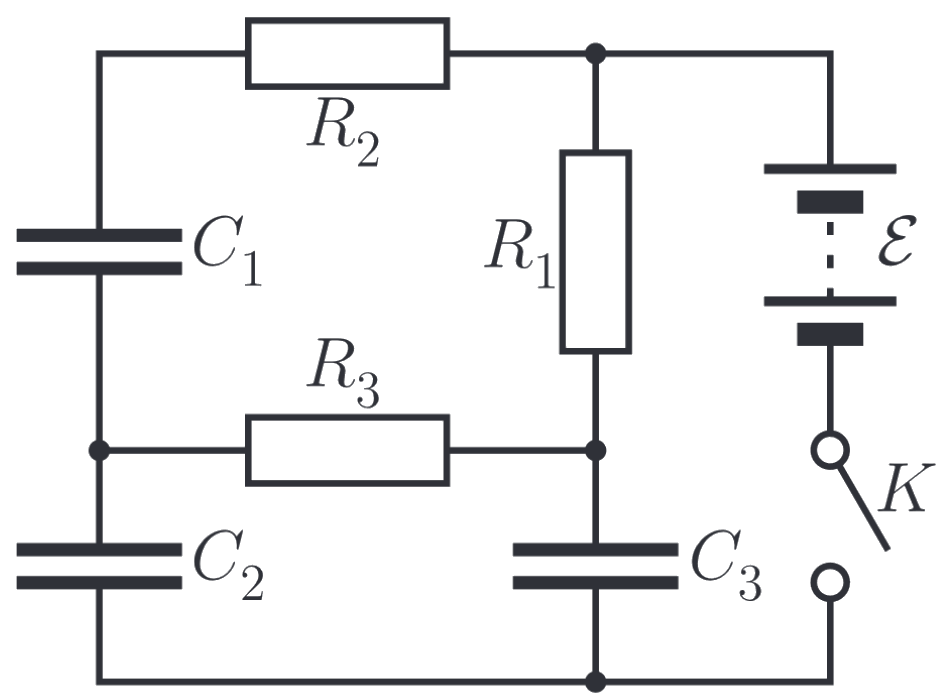
\includegraphics[width=0.43\textwidth]{S2 Figures/S2-45.png}
\end{center}
\end{solution}

\hypertarget{P46}{}
\begin{solution}{normal} % 46
A resistor $R$ and a capacitor $C$ are connected in series with a DC voltage source with emf $\mathcal{E}$. The capacitor was initially uncharged. Find the power dissipated by the resistor. (Kalda Circuits P57)
\end{solution}

\hypertarget{P47}{}
\begin{solution}{normal} % 47
A capacitor with capacitance $C=10\;\mu\text{F}$ is charged to a potential difference of $U_0=6\;\text{V}$. Then, a switch completes a circuit containting only the capacitor and a diode with current-voltage characteristic (let $U_d=1\;\text{V}$) shown in the graph below. How much energy is released at the switch in the form of a flash (i.e. arcing), if we neglect heat dissipation in the wires?
\begin{center}
    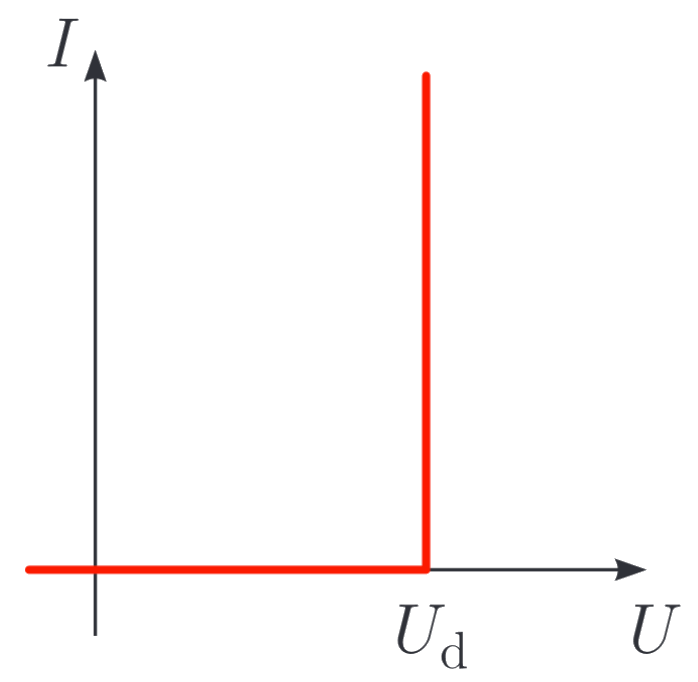
\includegraphics[width=0.32\textwidth]{S1 Figures/S1-35-2.png}
\end{center}
\end{solution}

\hypertarget{P48}{}
\begin{solution}{normal} % 48
Prove that the formula for the total capacitance of capacitors in series is given by
$$C=\left(\dfrac{1}{C_1}+\dfrac{1}{C_2}+\cdots\right)^{-1}$$
(Kalda Circuits P60)
\end{solution}

\hypertarget{P49}{}
\begin{solution}{normal} % 49
Three identical uncharged capacitors of capacitance $C$ are connected in series. A battery of emf $\mathcal{E}$ is connected to the circuit as shown. When the capacitors are fully charged, they are disconnected from the voltage source and connected to two identical resistors of resistance $R$ as shown in the circuit below. Determine the power dissipated by each resistor. (Kalda Circuits P61)
\begin{center}
    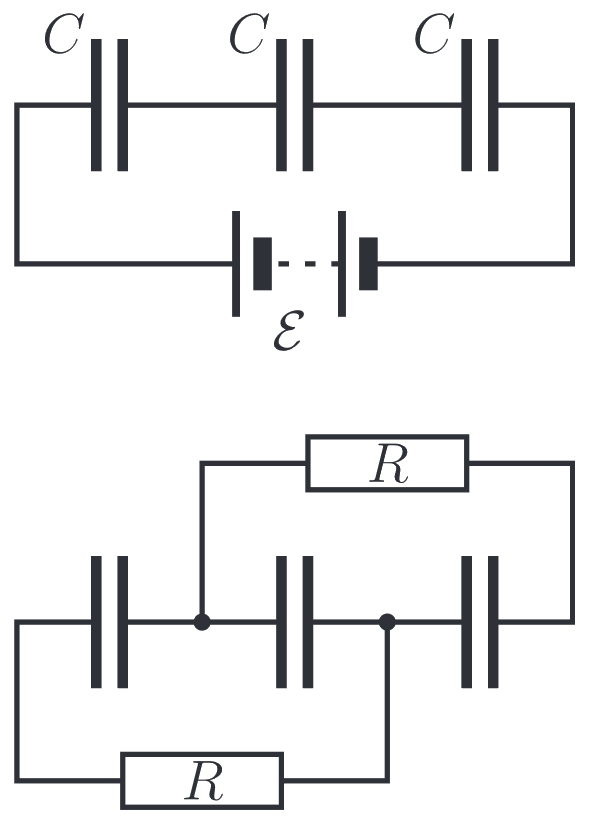
\includegraphics[width=0.33\textwidth]{S2 Figures/S2-49.png}
\end{center}
\end{solution}

\hypertarget{P50}{}
\begin{solution}{normal} % 50
In the circuit below, switch $K$ has been open for a long time. How much heat is dissipated at $R_1$ after closing the switch?
\begin{center}
    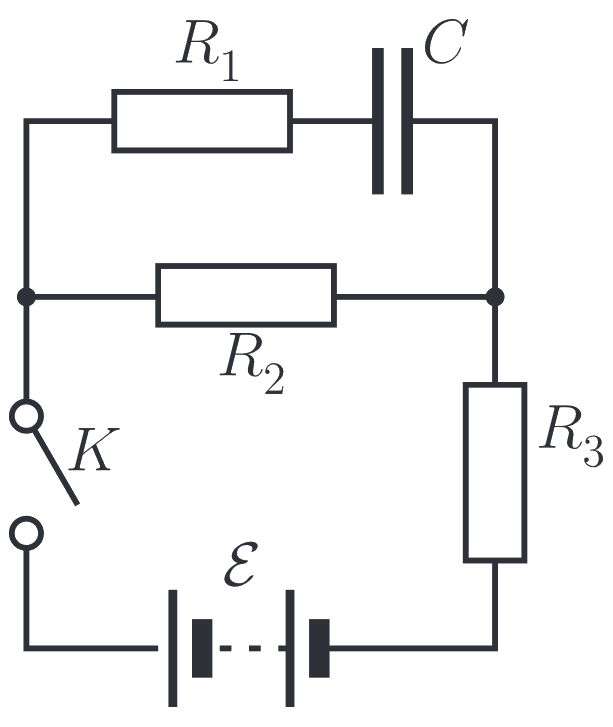
\includegraphics[width=0.33\textwidth]{S2 Figures/S2-50.png}
\end{center}
\end{solution}

\hypertarget{P51}{}
\begin{solution}{normal} % 51
Two parallel metal plates of area $100\;\text{cm}^2$ are spaced $1\;\text{mm}$. The plates are connected to a voltage source of emf $12\;\text{V}$. How much force is required to hold the plates in place? \textit{Note:} Use two different methods to solve the problem: in one case the voltage source is permanently connected; in the other case, once the capacitor is fully charged, the source is disconnected after the capacitor is fully charged. In either case, the answer should be the same. 
\end{solution}

\hypertarget{P52}{}
\begin{solution}{normal} % 52
A capacitor consists of two semicircular parallel plates that can rotate frictionlessly around a common axis (see the figure below). The distance between the plates is $d$ and each plate has radius $R$ ($d\ll R$). Determine the torque applied by the lower plate on the upper plate when the angle of overlap of the two plates is $\alpha$ ($\alpha\gg d/R$) and a voltage $U$ is applied to the plates.
\begin{center}
    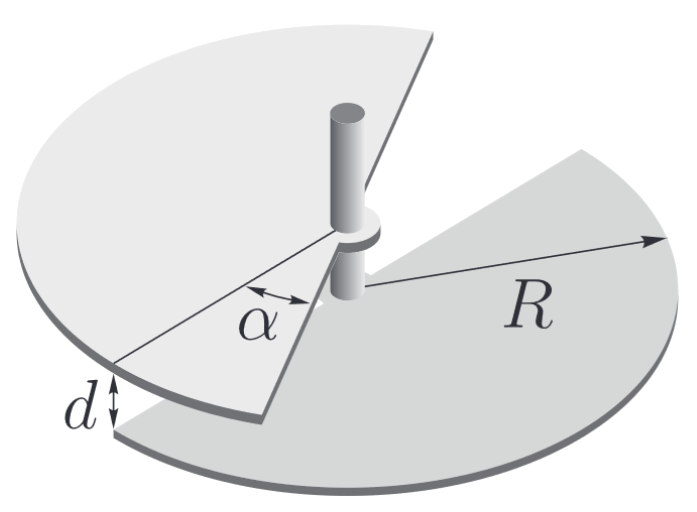
\includegraphics[width=0.32\textwidth]{S2 Figures/S2-52.png}
\end{center}
\end{solution}

\hypertarget{P53}{}
\begin{solution}{normal} % 53 ? unsure about translation
Find the minimum force necessary to remove a dielectric completely filling the space between two plates of a capacitor if the width of the plate is $a$, the distance between the plates is $d$, the dielectric constant is $\kappa$, and a voltage $U$ is applied to the capacitor.
\end{solution}

\hypertarget{P54}{}
\begin{solution}{normal} % 54
A parallel plate capacitor has plates spaced a distance $d$ apart. A voltage $U$ is applied across the capacitor. The capacitor is placed, along its lower edge, in a liquid with dielectric constant $\kappa$ and density $\rho$. How high does the liquid rise between the plates of the capacitor? Do not consider surface tension.
\end{solution}

\hypertarget{P55}{}
\begin{solution}{normal} % 55
The space between the plates of a capacitor is filled with an insulator with dielectric constant $5$ and resistivity $10^{12}\;\Omega\;\text{m}$. Find the time constant of the capacitor.
\end{solution}

\hypertarget{P56}{}
\begin{solution}{normal} % 56
The figure below shows the schematic for a simple timer. Assume that the inputs of the comparator consume practically no current. The capacitor is initially uncharged. How long does it take for the alarm to go off after closing the switch? \textit{Note:} The triangular circuit element is a comparator - a device that emits a signal (which in turn triggers an alarm) as soon as the potential difference between its inputs becomes positive. Dashed lines indicate connections between the comparator and alarm, but this is not required to solve the problem.
\begin{center}
    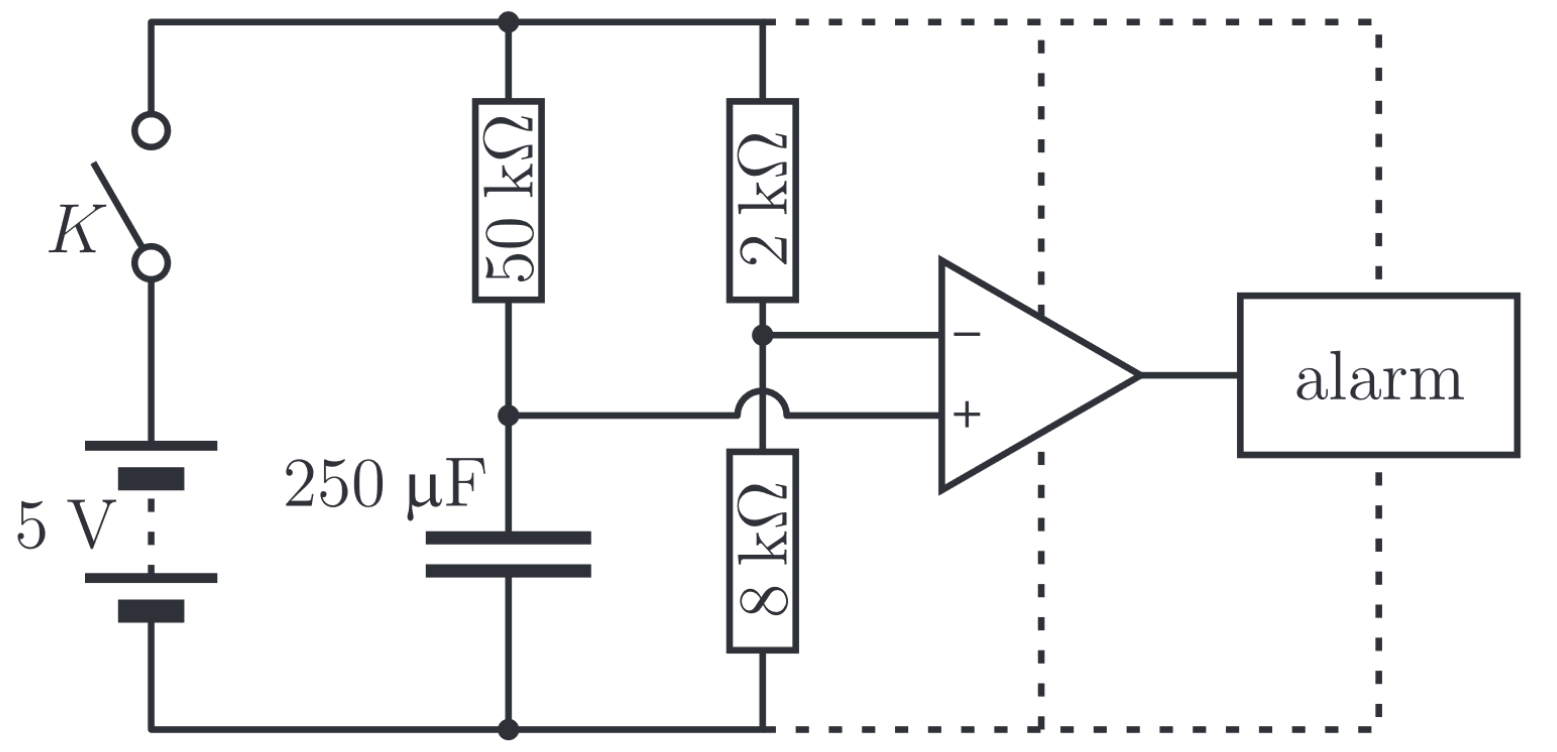
\includegraphics[width=0.53\textwidth]{S2 Figures/S2-56.png}
\end{center}
\end{solution}

\hypertarget{P57}{}
\begin{solution}{normal} % 57
Find the time constant of the capacitor in the diagram below after closing switch $K$.
\begin{center}
    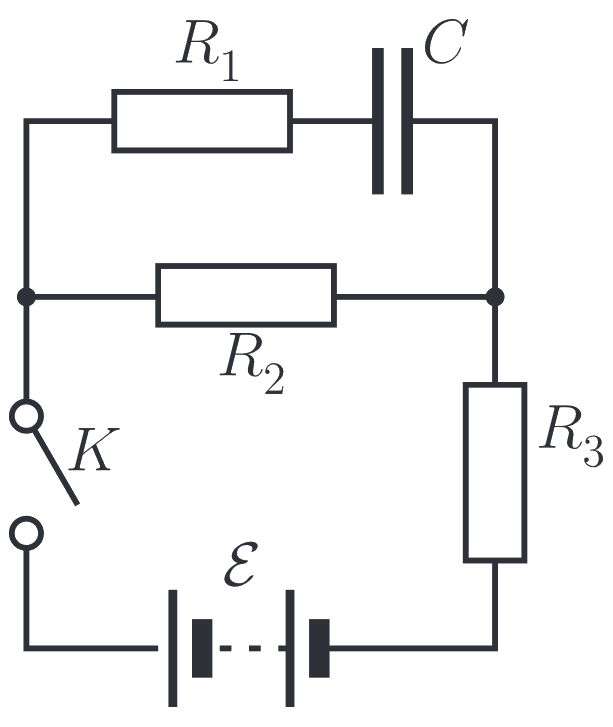
\includegraphics[width=0.33\textwidth]{S2 Figures/S2-50.png}
\end{center}
\end{solution}

\hypertarget{P58}{}
\begin{solution}{normal} % 58
An AC voltage as shown below is applied to a circuit consisting of a resistor and a capacitor connected in series. Determine the power dissipated by the resistor in the following cases: a) $T\ll RC$; b) $T\gg RC$.
\begin{center}
    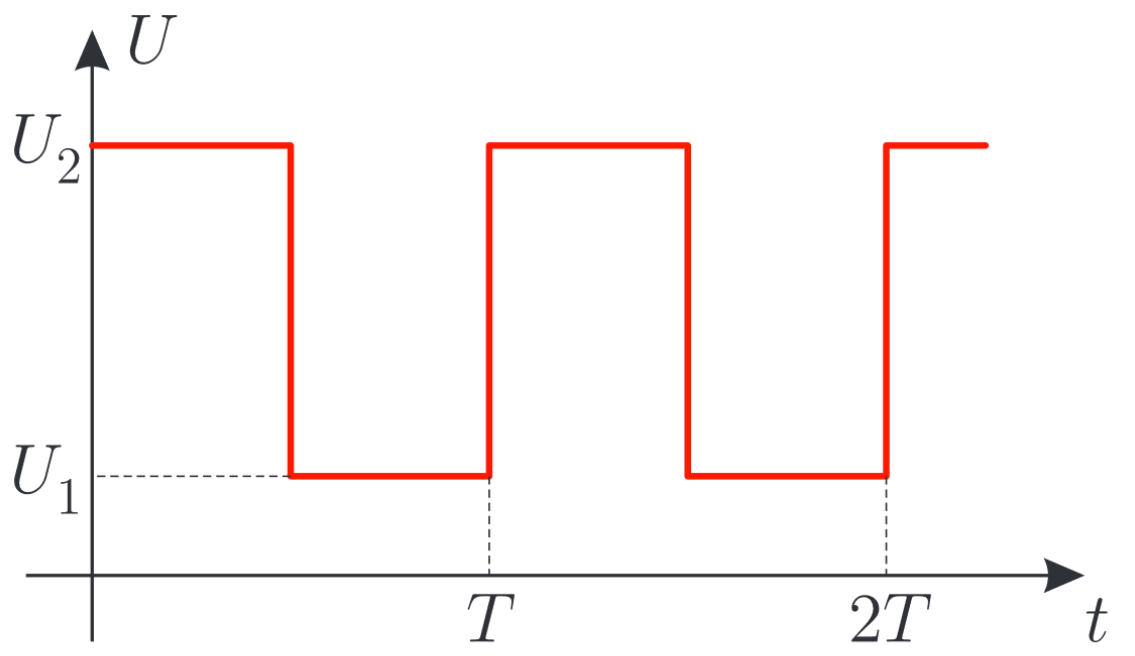
\includegraphics[width=0.5\textwidth]{S2 Figures/S2-58.png}
\end{center}
\end{solution}

\hypertarget{P59}{}
\begin{solution}{normal} % 59
A time-dependent current flows through a circuit consisting of a resistor and a capacitor connected in series. Determine the amplitude of voltage fluctuations in the capacitor in the following cases: a) $T\ll RC$; b) $T\gg RC$.
\begin{center}
    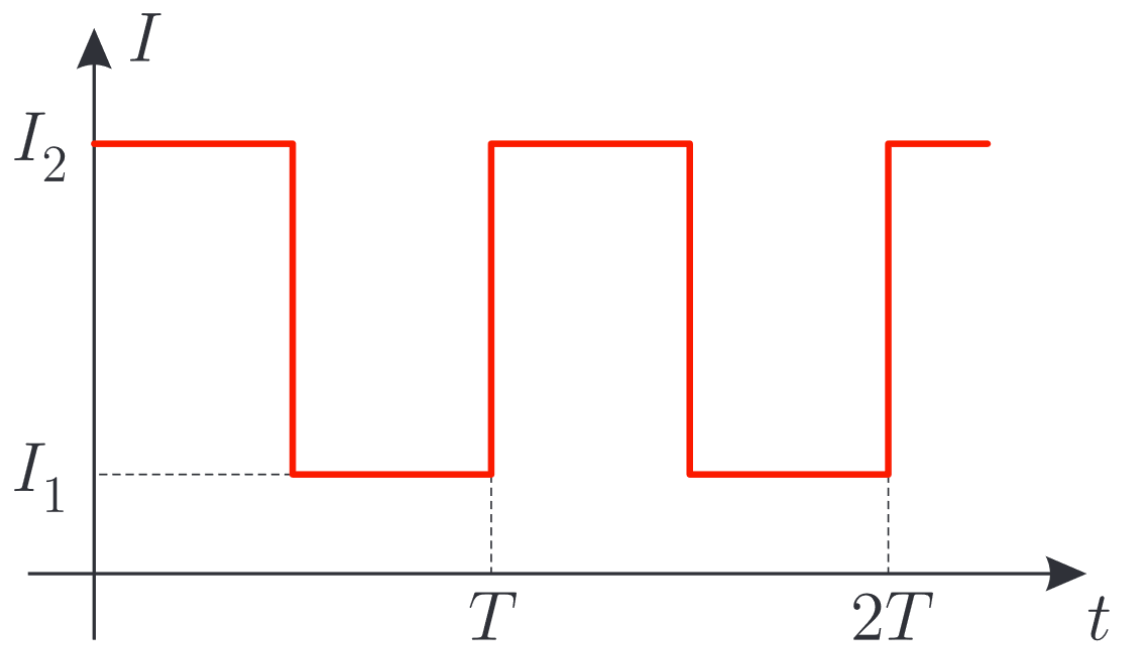
\includegraphics[width=0.5\textwidth]{S2 Figures/S2-59.png}
\end{center}
\end{solution}

\hypertarget{P60}{}
\begin{solution}{normal} % 60
A boy wants to build decorative lights using 50 LEDs, to be fed by AC voltage $V=V_0\cos(2\pi\nu t)$, with $V_0= 220\;\text{V}$ and $\nu= 50\;\text{Hz}$.  The circuit he plans to use is given below. The voltage of his LEDs can be taken to be equal to $3\;\text{V}$ (it remains constant for a wide range of forward currents); the nominal current is $20\;\text{mA}$. Find a) the optimal value of the resistor $R$ (ensuring a nominal operation of the diodes) and the power it dissipates, and b) the minimal value of the capacitance $C$, if the current fluctuations need to be less than 5\%. The rectifying diode $D$ can be considered to be ideal. (Kalda Circuits P75)
\begin{center}
    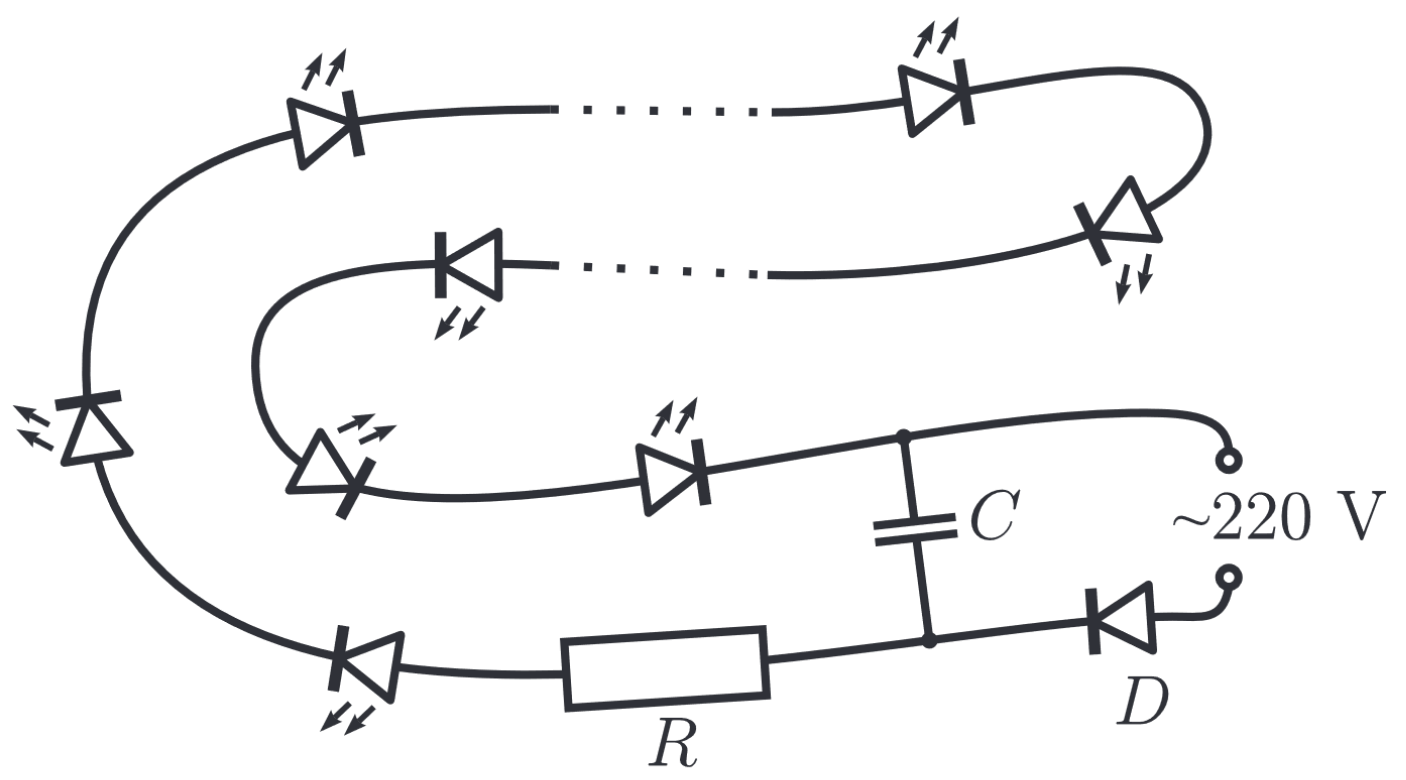
\includegraphics[width=0.7\textwidth]{S2 Figures/S2-60.png}
\end{center}
\end{solution}